\documentclass[10pt]{exam}
\usepackage[hon]{template-for-exam}
\usepackage{endnotes,graphicx}
\usepackage{tikz,graphicx,enumitem,multicol,float,my-tikz-clipart,silence,cclicenses,tikzpingus}
\graphicspath{{./figures/}}
\WarningFilter{latex}{Label `part}
\WarningFilter{latex}{There were multiply-defined labels}
\usetikzlibrary{arrows.meta}

\footer{}{\thepage}{\sc \myclass}


%\def\answer#1{\footnotetext{#1}}
%\def\myquestion{\item\stepcounter{footnote}}

\def\enoteheading{}
\def\answer#1{\endnotetext{#1}}
\def\theanswers{\theendnotes}
\def\myquestion{\item\stepcounter{endnote}}

\newenvironment{myquestions}{
  \begin{multicols}{2}\begin{enumerate}[resume]
}{
  \end{enumerate}\end{multicols}
}
\makeatletter
\patchcmd{\enit@setresumekeys}{\def}{\gdef}{}{}
\patchcmd{\enit@setresumekeys}{\def}{\gdef}{}{}
\makeatother

\newcommand{\myheading}[1]{\uplevel{\section*{#1}}
}
\newcommand{\mysubheading}[1]{\uplevel{\subsection*{#1}}
}

%uncomment if running Pandoc
% \renewcommand{\myheading}[1]{{\section*{#1}}}
% \renewcommand{\mysubheading}[1]{\subsection*{#1}}

\title{Chapter 4-5 Homework A (Dynamics)}
\author{Rohrbach}
\date{\today}

\def\mymaketitle{
  \begin{flushleft}
    {\LARGE \textbf \mytitle \par}
  \end{flushleft}
}

\newcommand{\bs}[2]{\textbf{#1} (\sc #2 Points)}


\newcommand{\GFig}[2]{  
  \begin{figure}[H]
    \centering
    \includegraphics[width=#2]{11_#1_Figure.jpg}
    \caption{Giancolli Figure 11-#1.}
    \label{11-#1}
  \end{figure}
}


\begin{document}
\maketitle

\vfill

\begin{center}
  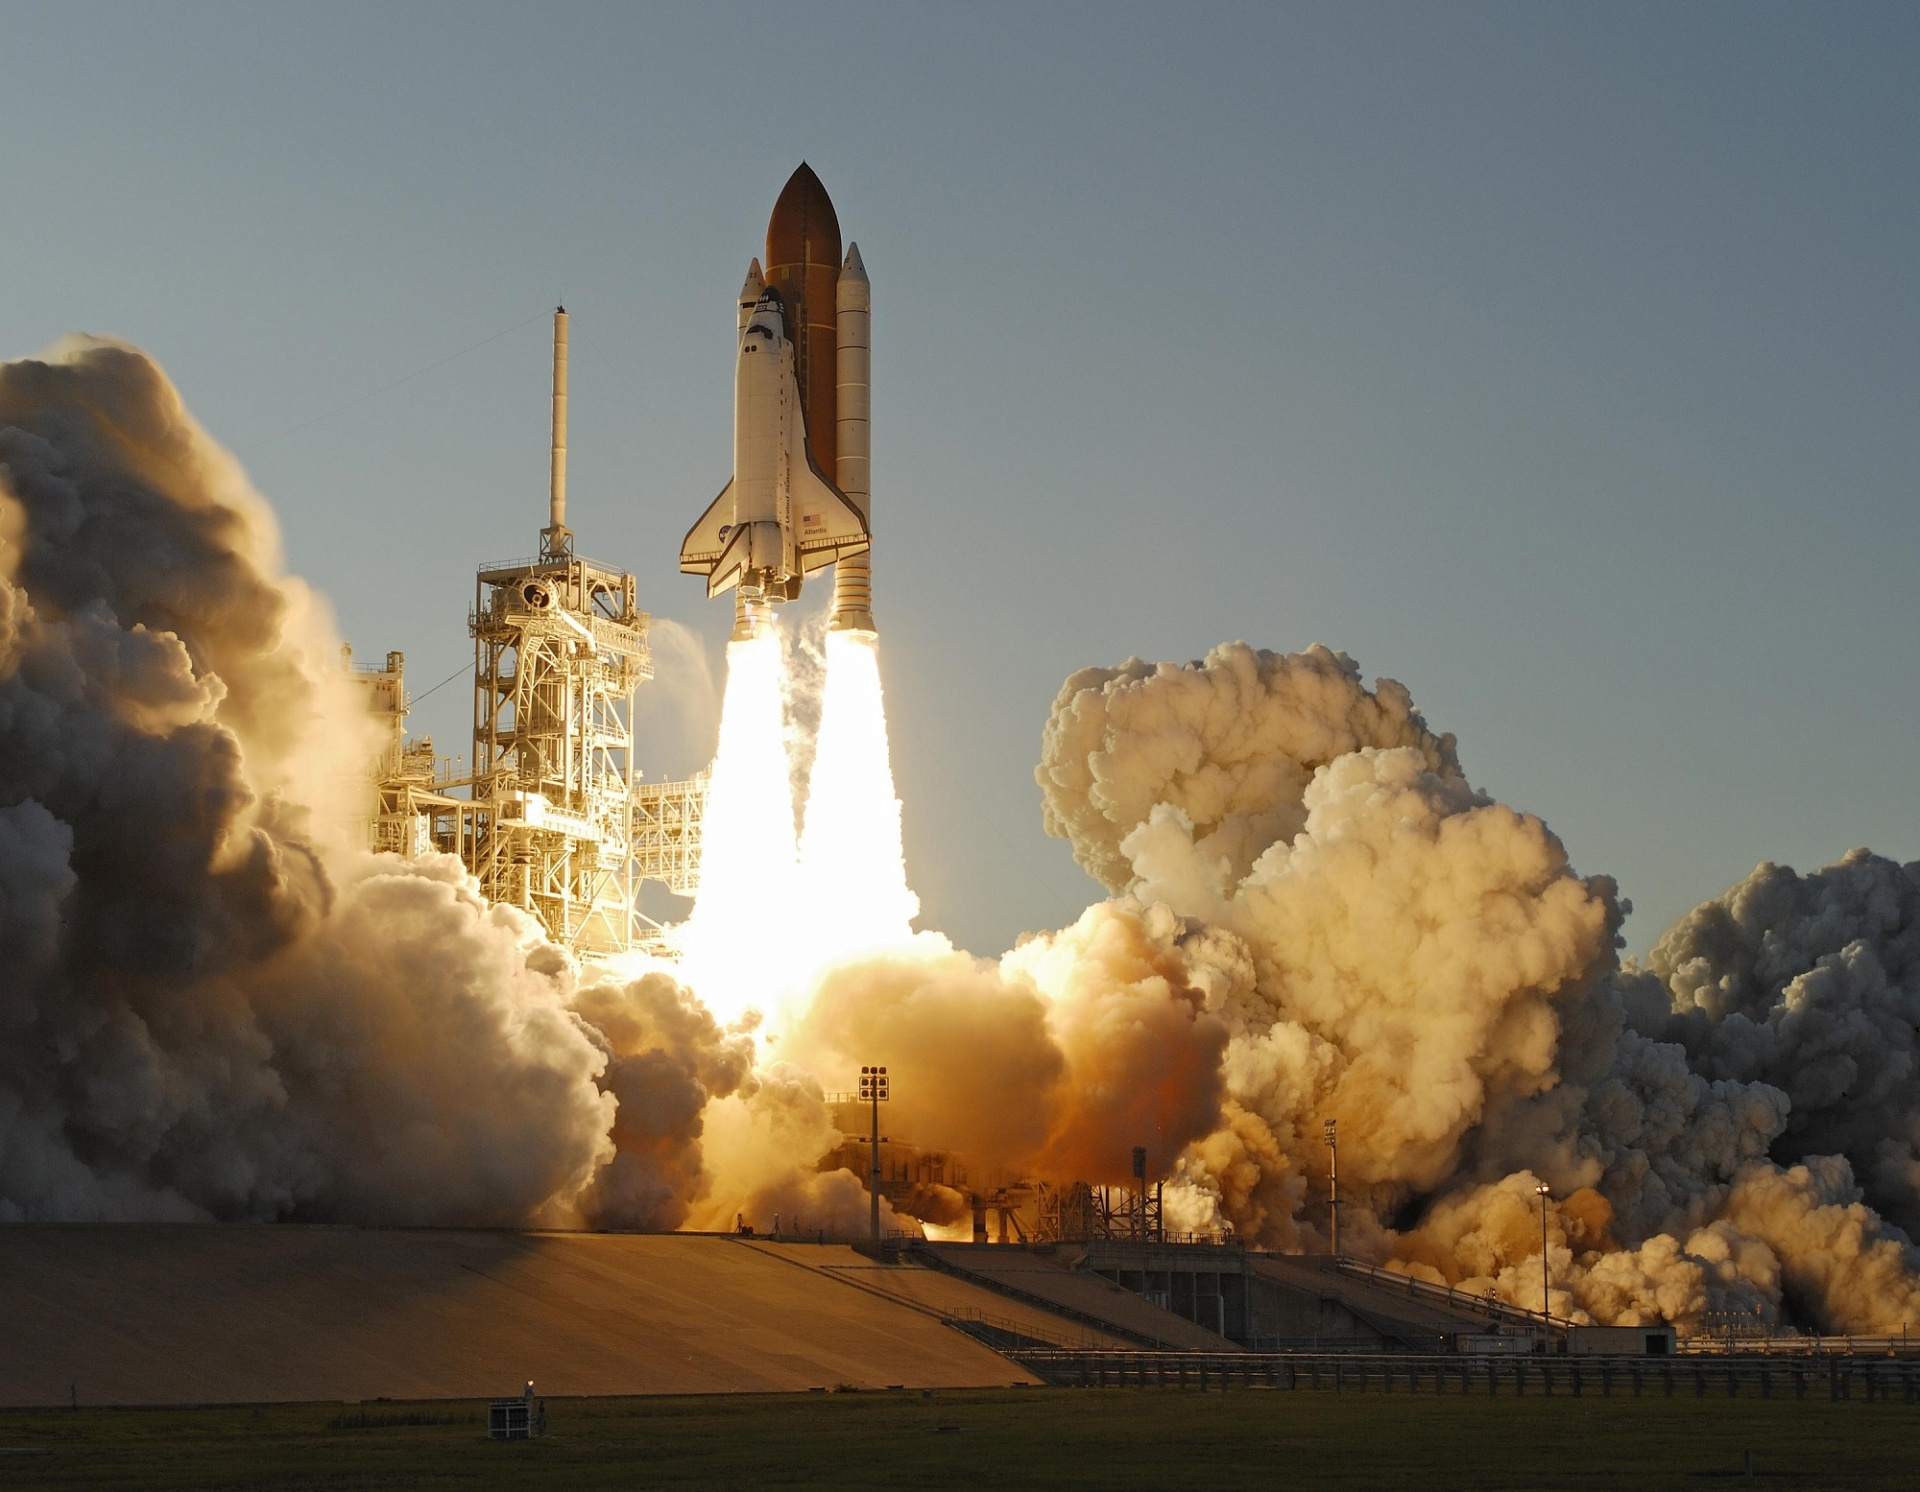
\includegraphics[width=5in]{OpenStaxImages/space-shuttle-launch}
\end{center}
  


  \vfill
  \hrule
  \vspace{0.2em}

  \section*{Equations}

  \begin{align*}
    \Sigma \vec{F} &= m\vec{a} &
    F_G &= mg &
    F_{f,s} &\le \mu_s F_N &
    F_{f,k} &= \mu_k F_N
  \end{align*}


  \hrule

  \section*{Selected Answers}

  \renewcommand{\enotesize}{\normalsize}
  \renewcommand{\enoteformat}{%
    \leftskip=1.8em
    \makebox[0pt][r]{\theenmark. }%
  }

  \hfill

  \begin{multicols}{2}
    \theanswers
  \end{multicols}



\pagebreak

\noindent
\textit{Questions and figures are from OpenStax} College Physics, \textit{2nd ed (Chapter 4) unless otherwise noted.}

\section*{Forces \& Newton's Laws}



\begin{myquestions}

\myquestion 
    (P1) A 63.0-kg sprinter starts a race with an acceleration of 4.20 m/s$^2$. What is the net external force on him? \answer{265 N}

  % \myquestion 
  %   (P2) If the sprinter from the previous problem accelerates at that rate for 20 m, and then maintains that velocity for the remainder of the 100-m dash, what will be his time for the race? \answer{9.26 s (a record!)}

  \myquestion
    (P10) A powerful motorcycle can produce an acceleration of 3.50 m/s$^2$ while traveling at 90.0 km/h. At that speed the forces resisting motion, including friction and air resistance, total 400 N. What is the magnitude of the force the motorcycle exerts on the ground to produce its acceleration if the mass of the motorcycle with rider is 245 kg? \answer{1260 N} 


\end{myquestions}

\vs[4]

\section*{Forces Conceptual Questions}

\begin{enumerate}[resume]
    \myquestion (CQ2) What properties do forces have that allow us to classify them as vectors? \vs
    \myquestion (CQ3) How are inertia and mass related? \vs
    %\myquestion (CQ4) What is the relationship between weight and mass? Which is an intrinsic, unchanging property of a body? \vs
    \myquestion (CQ5) Which statement is correct? (a) Net force causes motion. (b) Net force causes change in motion. Explain your answer and give an example. \vs
    %\myquestion (CQ6) Why can we neglect forces such as those holding a body together when we apply Newton's second law of motion? \vs
    %\myquestion (CQ8) \hfill Describe a situation in which the net external force on a system is not zero, yet its speed remains constant. \vs
    %\myquestion (CQ10) A rock is thrown straight up. What is the net external force acting on the rock when it is at the top of its trajectory? \vs
    \myquestion (CQ15) When you take off in a jet aircraft, there is a sensation of being pushed back into the seat. Explain why you move backward in the seat—is there really a force backward on you? (The same reasoning explains whiplash injuries, in which the head is apparently thrown backward.) \vs
    
    \pagebreak
    \myquestion (CQ18) Why does an ordinary rifle recoil (kick backward) when fired? The barrel of a recoilless rifle is open at both ends. Describe how Newton's third law applies when one is fired. Can you safely stand close behind one when it is fired? \vs
    \myquestion (Original Question) A horse pulls a cart with a force of 400 Newtons forward.  However, according to Newton's Third Law, whenever the horse pulls the cart, there is an equal and opposite reaction of the cart pulling the horse of 400 N backwards.  Why do these two forces not cancel each other out giving to a net force of zero?

    \tikzstyle{wheel}=[line width=10pt, fill=white]

    \begin{figure}[ht]
      \centering
      \begin{tikzpicture}[scale=0.3]
        \pingu[on horse,body=white, body front=white,small size, left eye color=white, right eye color=white,feet color=brown,bill color=white]
        \draw[rounded corners, fill=gray] 
          (0,-2) rectangle ++(7,-0.5);
        \draw[rounded corners, fill=gray] 
          (6,-1) -- ++(7,0) -- ++(-1,-4) -- ++(-5,0) -- cycle;
        \draw[wheel] (7,-5) circle (1);
        \draw[wheel] (12,-5) circle (1);
        \fill[pattern=north east lines] (-6,-6.3) rectangle ++(21, -0.5);
      \end{tikzpicture}
      \caption{(Original Diagram) A horse and cart.}
      \label{horse-cart}
    \end{figure}

    \vs

    \myquestion (Original Question) According to Newton's Third Law, when you jump off a desk, the force the Earth exerts on you, is equal to the force you exert on the Earth. However, it seems as if only you accelerate down. The earth doesn't seem to accelerate up. Why is this? \vs
    \myquestion (Original question) If a large semi-truck gets into a head-on collision with a small car, which vehicle experiences the larger force?  Which vehicle experiences the larger acceleration? \vs
  \end{enumerate}


\pagebreak

\section*{Single-Body Problems}

\begin{myquestions}

  \myquestion \answer{\SI{16500}{N}}
    (Original Question) A loaded semi truck has a mass of \SI{36000}{kg}.  Its engine applies a forward force of \SI{20820}{N}, causing it to accelerate at \SI{0.12}{m/s^2}.  Calculate the force of friction on the truck.

  \myquestion \answer{(a) 75 N; (b) 1.1 m}
    (P5) In Figure~\ref{4-7} below, the net external force on the 24-kg mower is stated to be 51 N. (a) If the force of friction opposing the motion is 24 N, what applied force (in newtons) is the person exerting on the mower? (b) Suppose the mower is moving at 1.5 m/s when the applied force is removed. How far will the mower go before stopping? 
    %
    \begin{figure}[H]
      \centering
      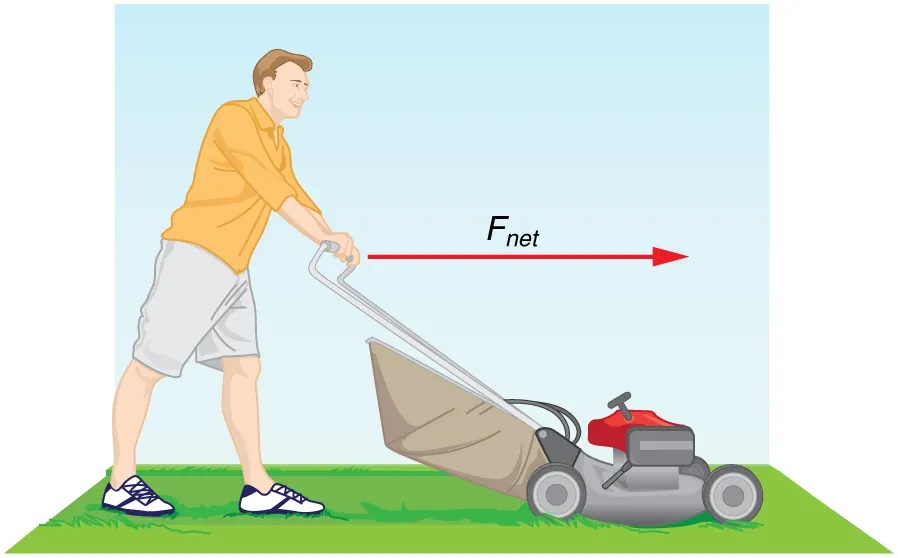
\includegraphics[width=2in]{OpenStaxImages/4-7.jpg}
      \caption{(OpenStax Fig 4.7) The net force on a lawn mower is 51 N to the right.}
      \label{4-7}
    \end{figure}
  

  \myquestion \answer{(b) \SI{0.130}{m/s^2}; (c) \SI{0}{m/s^2}} 
    (P9) Suppose two children push horizontally, but in exactly opposite directions, on a third child in a wagon. The first child exerts a force of 75.0 N, the second a force of 90.0 N, friction is 12.0 N, and the mass of the third child plus wagon is 23.0 kg. (a) Draw a free-body diagram, including all forces acting on the system. (b) Calculate the acceleration. (c) What would the acceleration be if friction were 15.0~N?

  
  \myquestion 
    (P13) The weight of an astronaut plus their space suit on the Moon is only 250~N. How much do they weigh on Earth? What is the mass on the Moon? On Earth? (The acceleration of gravity on the moon is 1.62 m/s$^2$) \answer{1500 N}

  \myquestion
    (P14) Suppose the mass of a fully loaded module in which astronauts take off from the Moon is 10,000 kg. The thrust of its engines is 30,000 N and the acceleration of gravity on the moon is 1.62 m/s$^2$. (a) Calculate its the magnitude of acceleration in a vertical takeoff from the Moon. (b) Could it lift off from Earth? If not, why not? If it could, calculate the magnitude of its acceleration. \answer{(a) \SI{1.38}{m/s^2}; (b) cannot take off}

  \myquestion \answer{737.0 N}
    (Original Question) You are standing on a scale in an elevator.  If your mass is 67~kg, what force would the scale read if the elevator accelerates up at a rate of 1.2~m/s$^2$?  Remember, a scale measures normal force, not weight.  Make sure to draw and label the free-body diagram. 

\end{myquestions}





\pagebreak

\section*{Multi-Body Problems}

\begin{myquestions}
  
\myquestion
     (P22) Consider the baby being weighed in Figure~\ref{4-33}. (a) What is the mass of the child and basket if a scale reading of 55 N is observed? (b) What is the tension $T_1$ in the cord attaching the baby to the scale? (c) What is the tension $T_2$ in the cord attaching the scale to the ceiling, if the scale has a mass of 0.500 kg? The masses of the cords are negligible. \answer{(a) \SI{5.6}{kg}; (b) \SI{55}{N}; (c) 60 N}

      \begin{figure}[H]
        \centering
        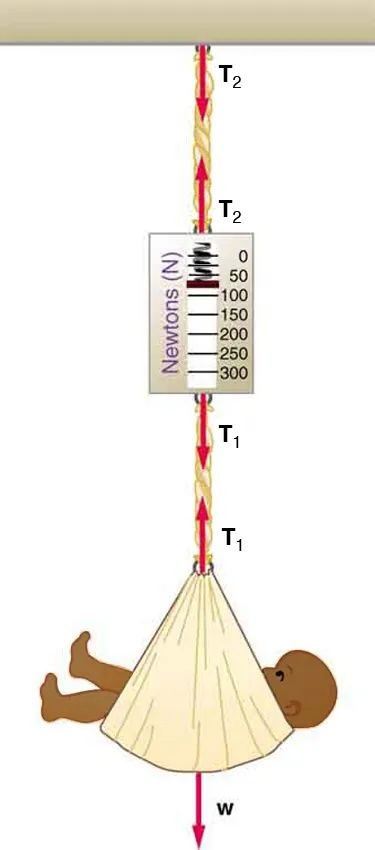
\includegraphics[height=2.5in]{OpenStaxImages/4-33.jpg}
        \caption{(OpenStax Fig 4-33) A baby is weighed using a spring scale.}
        \label{4-33}
      \end{figure}

  

  \tikzstyle{box}=[rounded corners,draw,minimum height=1cm]

  \myquestion \label{Atwood}
    (Original question) Two blocks of masses $m_1=5.0$~kg and $m_2=3.0$~kg are connected by a light, inextensible string that passes over a frictionless pulley. The system is released from rest. \answer{(b) \SI{2.45}{m/s^2}; (c) \SI{36.75}{N}}
    %
    \begin{parts}
      \part Draw a free-body diagram for each block.
      \part Determine the acceleration of the system.
      \part Find the tension in the string.
    \end{parts}

    \begin{figure}[H]
      \centering
      \begin{tikzpicture}
        \node[box] (one) at (-.75,0) {$m_1$};
        \node[box] (two) at (.75,-0.5) {$m_2$};
        \draw[very thick] (one.north) -- (-.75,3) 
          arc (180:0:.75) -- (two.north);
        \draw[very thick] (0,3) circle[radius=.75];
      \end{tikzpicture}
      \caption{(Original Diagram) Figure for problem~\ref{Atwood}.}
    \end{figure}
\end{myquestions}

  \pagebreak

\begin{myquestions}
  
  \myquestion \label{hero1}
     (P34) Figure~\ref{4-38} shows Superhero and Trusty Sidekick hanging motionless from a rope. Superhero's mass is 90.0 kg, while Trusty Sidekick's is 55.0 kg, and the mass of the rope is negligible. (a) Draw a free-body diagram of the situation showing all forces acting on Superhero, Trusty Sidekick, and the rope. (b) Find the tension in the rope above Superhero. (c) Find the tension in the rope between Superhero and Trusty Sidekick. Indicate on your free-body diagram the system of interest used to solve each part. \answer{(b) \SI{1420}{N}; (c) 539 N}

    
  \myquestion \label{hero2}
    (Original question) The top rope in Figure~\ref{4-38} is attached to the bottom of an elevator that begins to accelerate upward.  The tension of the top rope increases to 1600~N. (a) Calculate the tension on the rope between Superhero and Trusty Sidekick. (b) Calculate the acceleration of the two heroes. \answer{(a) \SI{607}{N}; (b) \SI{1.23}{m/s^2}}


    \begin{figure}[H]
      \centering
      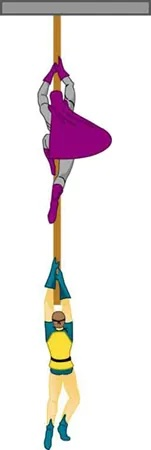
\includegraphics[height=2.5in]{OpenStaxImages/4-38.jpg}
      \caption{(OpenStax Fig 4-38) For problems~\ref{hero1}~\&~\ref{hero2}.  Superhero (at the top) is 90.0~kg; Trusty Sidekick (on the bottom) is 55.0~kg.  The ropes are massless.}
      \label{4-38}
    \end{figure}


\end{myquestions}




\pagebreak

\section*{Dynamics Conceptual}

\begin{enumerate}[resume]
  \myquestion (CQ23)  To simulate the apparent weightlessness of space orbit, astronauts are trained in the hold of a cargo aircraft that is accelerating downward at $g$. (a) Why will they appear to be weightless, as measured by standing on a bathroom scale, in this accelerated frame of reference? (b) Is there any difference between their apparent weightlessness in orbit and in the aircraft? \vs

    \myquestion (Original Question) \label{compare-q} Consider the two boxes of masses $m_1 > m_2$ attached to each other by a massless cord shown in Figure~\ref{compare-fig}.  In both cases, the system is pulled by 75~N of force.  In which orientation is the tension force larger?  Explain.  You may neglect friction.
    
    \tikzstyle{box}=[rounded corners,draw,minimum height=1cm]
    \begin{figure}[h]
      \centering
      \begin{tikzpicture}
        \begin{scope}
            \node at (-1.5,0) {(a)};
            \node[box] (two) at (3,0) {$m_2$};
            \draw[very thick] (two) -- (0,0);
            \node[box,minimum width=1.5cm,minimum height=1.5cm,fill=white] (one) at (0,0.25) {$m_1$};
            \fill[pattern=north east lines] (-1,-0.5) rectangle
              ++(6,-0.25);
            \draw (-1,-0.75) -- ++(0,0.25) -- 
              ++(6,0) -- ++(0,-0.25); 
            \draw[-{Stealth},ultra thick,orange] (two.east) 
              ++(0,0.2) -- ++(1,0) node[above] {75 N};
        \end{scope}

        \begin{scope}[shift={(0,-3)}]
            \node at (-1.5,0) {(b)};
            \node[box] (two) at (0,0) {$m_2$};
            \draw[very thick] (two) -- (3,0);
            \node[box,minimum width=1.5cm,minimum height=1.5cm,fill=white] (one) at (3,0.25) {$m_1$};
            \fill[pattern=north east lines] (-1,-0.5) rectangle
              ++(6,-0.25);  
            \draw (-1,-0.75) -- ++(0,0.25) -- 
              ++(6,0) -- ++(0,-0.25); 
            \draw[-{Stealth},ultra thick,orange] (one.east) 
              ++(0,0.2) -- ++(1,0) node[above] {75 N};
        \end{scope}

      \end{tikzpicture}
      \caption{(Original Diagram) Figure for \ref{compare-q}}
      \label{compare-fig}
    \end{figure}

    \vs

  \end{enumerate}


\pagebreak


\section*{Additional Practice}
These problems are not required and are not bonus. Worked out solutions are available on Schoology.
  
\begin{myquestions}
  
    \myquestion
      (Ch 4, P19 from Giancolli \textit{Physics: Principles with Applications}, 7th ed.) The cable supporting a 2125-kg elevator has a maximum strength of 21,750~N.  What maximum upward acceleration can it give without breaking? \answer{\SI{0.44}{m/s^2}}

    \myquestion
      (Ch 4, P25 from Giancolli)  One 3.2-kg paint bucket is hanging by a massless cord from another 3.2-kg paint bucket, also hanging by a massless cord, as shown in Figure~\ref{G4-49}.  (a) If the massless buckets are at rest, what is the tension on each cord?  (b) If the two buckets are pulled upward with an acceleration of \SI{1.25}{m/s^2} by the upper cord, calculate the tension on each cord. \answer{(a) 31.36 N and 62.72 N; (b) 35.36 N and 70.72 N}

      \begin{figure}[H]
        \centering
        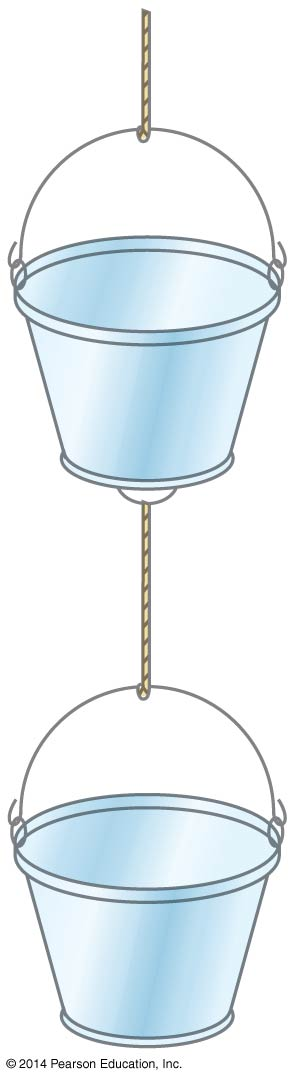
\includegraphics[height=1.9in]{OpenStaxImages/Giancolli4-49.jpg}
        \caption{Fig 4-49 from Giancolli}
        \label{G4-49}
      \end{figure}

    \myquestion
        (Ch 4, P49 from Giancolli, modified) Two crates of mass 65~kg and 125~kg are in contact and at rest on a horizontal surface (Figure~\ref{G4-47}).  A 650-N force is exerted on 65-kg crate.  Calculate (a) the acceleration of the system and (b) the force that each crate exerts on the other.  (c) Repeat with the crates reversed. \answer{(a) \SI{3.42}{m/s^2} (b) \SI{427.5}{N} (c) \SI{3.42}{m/s^2} and \SI{22.3}{N} }

        \begin{figure}[H]
          \centering
          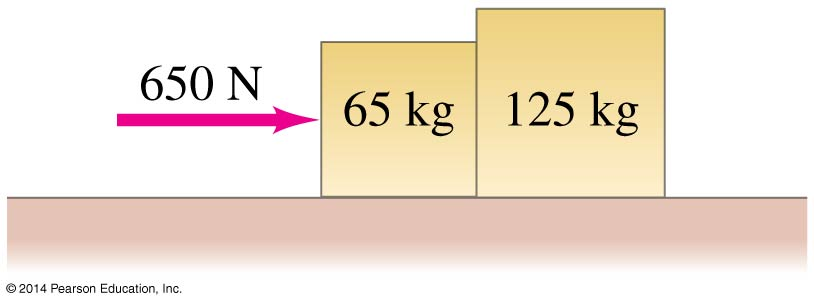
\includegraphics[width=2.5in]{OpenStaxImages/Giancolli4-57.jpg}
          \caption{Fig 4-47 from Giancolli}
          \label{G4-47}
        \end{figure}


\end{myquestions}

\hrule

\section*{Bonus}

You will be given bonus if you complete these problems \emph{on a separate sheet of paper}
  
\begin{myquestions}


\myquestion 
  \label{b1} (P44) When starting a foot race, a 70.0-kg sprinter exerts an average force of 650 N backward on the ground for 0.800 s. (a) What is his final speed? (b) How far does he travel?

\myquestion
  \label{b2} (P23) A $5.00\times10^5$-kg rocket is accelerating straight up. Its engines produce $1.250\times10^7$ N of thrust, and air resistance is $4.50\times10^6$ N. What is the rocket's acceleration? Explicitly show how you follow the steps in the Problem-Solving Strategy for Newton's laws of motion. 

  
\end{myquestions}

  
\end{document}